\documentclass[12pt, letterpaper]{article}
\usepackage[utf8]{inputenc}
\usepackage[margin=1in]{geometry}
\usepackage{graphicx}
\usepackage{amsmath}
\usepackage{nccmath}
\graphicspath{ {./Chem 156 Images/} }

\setlength{\parskip}{1em}
\setlength{\parindent}{0em}


\begin{document}
    \section*{Chapter 14: Sedimentation Velocity}
    The external force (on a per molecule basis) due to centrifugation is 
    \textbf{m$\phi\omega^2$r}, where \boldmath{$\phi$} is the \textbf{density increment}
    , \textbf{$\omega$} is the \textbf{angular velocity}, m is the 
    \textbf{mass}, and r is the \textbf{radius}. The \textbf{opposing frictional force} is 
    \textbf{-fv}. When setting the sum of these forces to zero (terminal velocity), 
    the equation yields: 

    \begin{equation}
        V = \frac{m\phi\omega^2 r}{f}
    \end{equation}

        or, on a per mole basis: 

    \begin{equation}
        V = \frac{M\phi\omega^2 r}{N_Af}
    \end{equation}

    How do you visualize velocity \textbf{v} in a velocity sedimentation experiment? If the
    sample begins with the macromolecule uniformly distributed (concentration is equal everywhere
    in tube), then when centrifugation begins, the \textbf{top region} (low r) of the sample will lose its 
    macromolecules.  

        
 
   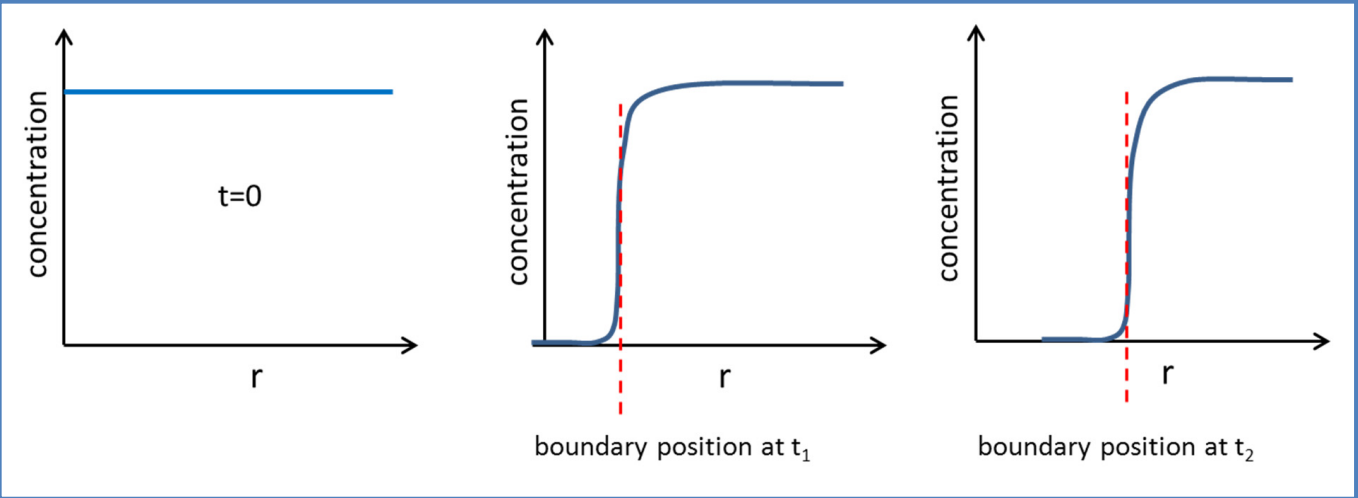
\includegraphics[scale = 0.70]{Sedimentaton Velocity with Radius.png}

    The sedimentation velocity $\textbf{v}$ is the speed of the boundary: \(\frac{\Delta r}{\Delta t} \) % need to do inline math here
    \\
    \\
    \\
    \\

    \subsection*{Meaning and Measurement of Sedimentation Coefficient, s}

    How does the sedimentation velocity \textbf{v} relate to molecular properties? From the equation
    \(V = \frac{M\phi\omega^2 r}{N_Af}\), v is affected by both molecular properties (M) and experimental
    parameters $(\omega)$. We want to separate the two kinds of variables on different sides of the equation: 

    \begin{equation}
        \frac{v}{\omega^2 r} = \frac{m\phi}{f}
    \end{equation}


    Now, introduce \textbf{sedimentation coefficient s} to be equal to those quantities. s is obtained experimentally using \(s = \frac{v}{\omega^2 r} \)
    s is obtained using molecular properties through:
    \begin{equation}
        s = \frac{M\phi}{N_Af} \; \text{ or } \useshortskip s = \frac{m\phi}{f}
    \end{equation}

    If angular velocity $\omega$ $\uparrow$, then the sedimentation velocity v $\uparrow$ from eq. (1). But the sedimentation coefficient s
    is unaffected. We know this is true becuase from \textbf{equation 4}, we can relate s to molecular properties without reference to 
    experimental parameters. 
    
    Since v is defined as \( \frac{dr}{dt}\) we can determine that: \\
    \begin{equation}
        s = \frac{\frac{dr}{dt} }{\omega^2 r} = \frac{\frac{dln(r)}{dt}}{\omega^2}
    \end{equation}

    Measuring the position r of the boundary at a series of time points during the experiment and plotting them as 
    \textbf{ln(boundary position) vs. t}  should give a straight line with slope s$\omega^2$, which can be used to find s.

    A special unit is used to express the value of the sedimentation coefficient (natural units are seconds). 
    The \textbf{Svedberg, S} is defined as $10^{-13}$ sec. 

    \subsection*{Relating s to molecular properties}

    The sedimentation coefficient relates to molecular properties in two ways: 
    \begin{itemize}
        \item dependence on mass
        \item frictional coefficient f (which depends on size $\rightarrow$ mass)
    \end{itemize}

    Starting with \(s = \frac{m\phi}{f} \), where f = 6$\pi\eta$R $\rightarrow$ \(s = \frac{m\phi}{6\pi \eta R}\)

    But R relates to volume and mass according to \(V = \frac{4}{3} \pi R^3 \) $\rightarrow$ \(R = (\frac{3V}{4 \pi})^{\frac{1}{3}} \)

    Relate volume V to mass m by the density $\rightarrow$ m = V$\rho$ and substitute V for $\frac{m}{\rho}$

    \begin{align*}
        s &= \frac{m \phi}{6 \pi \eta (\frac{3m}{4 \pi \rho})^{\frac{1}{3}}} \\ \\
       s &= m^{\frac{2}{3}} (\frac{\phi}{6 \pi \eta}) (\frac{4 \pi \rho}{3})^{\frac{1}{3}}  \hbox{ or } s = (\frac{M}{N_A})^{\frac{2}{3}} (\frac{\phi}{6 \pi \eta})(\frac{4 \pi \rho}{3})^{\frac{1}{3}}
    \end{align*}

    Do larger molecules sediment move faster or slower than small molecules of equal density and similar shape? Centrifugal force on an object 
    is proportional to mass, but opposing force is only $\frac{1}{3}$ power of the mass. 
    
    So larger molecules move faster, according to $\frac{2}{3}$ power of their mass.

    \textbf{This assumes that the protein or molecule is nearly spherical since we used Stoke's Equation}. If 
    the molecule of interest is \textbf{non-spherical}, then it will have the same centrifugal force but $\uparrow$ frictional 
    force $\rightarrow$ $\downarrow$ sedimentation coefficient s. This will result in a lower estimation for molecular 
    weight. 

    \subsection*{Combining s and D (diffusion coefficient) to get molecular weight without a spherical assumption}

    We can eliminate the assumption of spherical shape if we have measured values for s and D together. Having both values 
    cancels frictional coefficient out. We know that \(f = \frac{K_B T}{D} \) and from equation (4), \(f = \frac{M \phi}{N_A s} \) 
    If we equate the two together: 

    \begin{align*}
        f = \frac{K_B T}{D} &= \frac{M \phi}{N_A s} \\ \\
        M &= (\frac{RT}{\phi})(\frac{s}{D})
    \end{align*}

    Molecular weight relates only to the ratio of s to D, shape is no longer considered (frictional coefficient). 
    
    \newpage
    The diffusion coefficient D can be obtained from the sedimentation experiment itself. Under ideal conditions without
    diffusion, the concentration profile at the boundary would be perfectly steep. At a position just before the boundary 
    layer, there will be no macromolecules. Right at the boundary layer, there will be a concentration of macromolecules
    that is the same all throughout the tube after that layer.  

    \begin{center}
        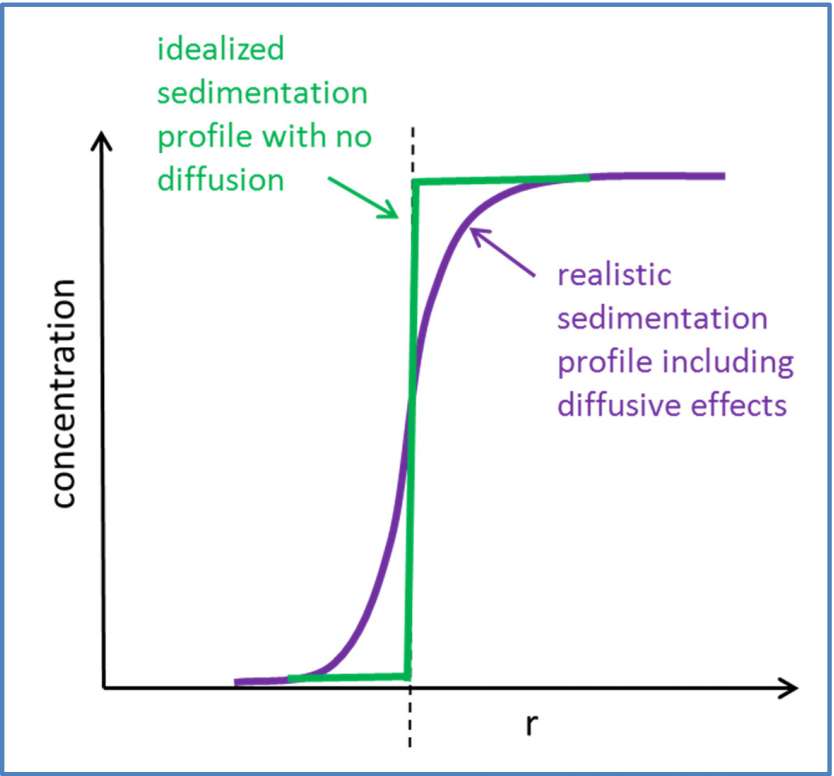
\includegraphics[scale = 0.70]{Sedimentation Profile.png}
    \end{center}

    \newpage

    \section*{Chapter 15: Chemical Reaction Kinetics}   
    \subsection*{Reaction Velocity, v}

    If we consider a reaction to be reactants $\rightarrow$ products, then reaction velocity v is the frequency
    (\#/time) wth which the event is occurring per unit volume. The units of v are \(\frac{\#}{volume \times time} \)
    or M/sec. There is only one velocity associated with the reaction, even though multiple reactants and products may be 
    involved. 

    The reaction velocity is indicated equally by the rate of change of \textbf{any} of the species involved:

    \begin{equation}
        \alpha A + \beta B + \dots \rightarrow \gamma C + \delta D + \dots
    \end{equation}
    \begin{align*}
        \frac{-d[A]}{dt} &= \alpha v \\
        \frac{-d[B]}{dt} &= \beta v \\
        \frac{-d[C]}{dt} &= \gamma v \\
        \frac{-d[D]}{dt} &= \delta v\\
    \end{align*}

    Rearranging to isolate velocity v gives \\
    
    \(v = - (\frac{1}{\alpha})(\frac{d[A]}{dt}) = (\frac{1}{\beta})(\frac{d[B]}{dt}) = (\frac{1}{\gamma})(\frac{d[C]}{dt}) = (\frac{1}{\delta})(\frac{d[D]}{dt}) = \dots \)
    
    Evidently, if we measure the rate of change of concentration of some species, then we measured reacton velocity v.

    \subsection*{Rate laws: how v depends on concentrations}
    Velocity of a reaction depends on how concentrated the reactants are. Besides concnetration, different reactions 
    (different chemical species) will have different v according to likelihood of underlying chemical events $\rightarrow$ k

    Combined dependence of v on rate constant k and concentrations $\rightarrow$ \textbf{rate law}. \\ \\

    Consider the equation: \(\mathrm{A} \stackrel{\mathrm{k}}{\longrightarrow} \mathrm{B} \)

    The rate law is \textbf{v = k[A]}, this reaction is first order in A. 

    Now consider \( 2\mathrm{A} \stackrel{\mathrm{k}}{\longrightarrow} \mathrm{B} \) $\Rightarrow$ \textbf{v = k[A]$^2$}, and the reaction is second order in A.
    


    If the equation is now \( \mathrm{A}+\mathrm{B} \stackrel{\mathrm{k}}{\longrightarrow} \mathrm{C} \), the rate law is now \textbf{v = k[A][B]}.

    \subsection*{Relationship of rate constants to equilibrium constants}

    What about if we had reversible processes? Velocities of forward and reverse reactions depend on the concentrations of 
    reactants and products, respectively. When the concentrations are reached where forward and reverse reactons are equal, 
    no \textbf{net} conversion is occurring. This is \textbf{chemical equilibrium}. Consider the reaction:

    \begin{equation}
        2 A \stackrel{k_1}{\underset{k_{-1}}{\rightleftharpoons}} B
    \end{equation}

    The \textbf{forward} reaction velocity is \textbf{v = k$_1$[A]$^2$} \\ \\
    The \textbf{reverse} reaction velocity is \textbf{v = k$_{-1}$[B]$^2$}


    At \textbf{equilibrium}, k$_1$[A]$^2$ = k$_{-1}$[B]$^2$ and \( \frac{k_1}{k_{-1}} = \frac{[B]}{[A]^2} \)

    The ratio of the rate constants is equal to the equilibrium constant K. 

    \subsection*{Integrating Rate Laws}

    For simple reactions, we can integrate the differential equations that come from rate law to describe how concentrations of reactants and products change over time

    \underline{1st Order Decay}
    
    \(\mathrm{A} \stackrel{\mathrm{k}}{\longrightarrow} \mathrm{B} \)

    To get a differential equation in terms of [A], combine two points: 
    \begin{itemize}
        \item First need \(v = \frac{-d[A]}{dt} \)
        \item Also need \(v = k[A] \)
    \end{itemize}

    \newpage

    If we equate them together, we get the following: 

    \begin{align*}
        \frac{-d[A]}{dt} &= k[A] \\ \\
        \int \frac{d[A]}{[A]} &= -k \int dt \\ \\
        \ln[A] |_{[A]_0} ^{[A]} &= -\left.k t\right|_0 ^t 
    \end{align*}

    This gives us the familiar first order decay equations
    \begin{equation}
        \ln(\frac{[A]}{[A]_0}) = -kt
    \end{equation}

    \begin{figure}[h]
        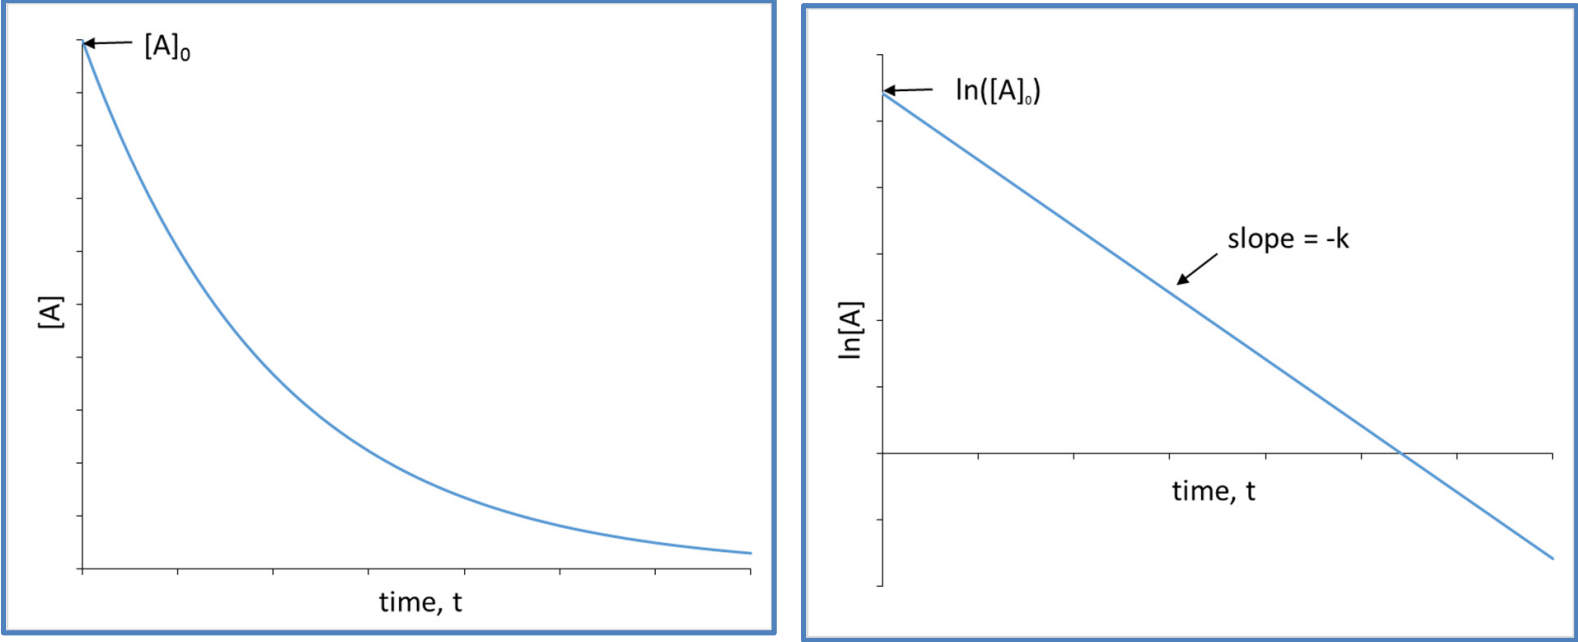
\includegraphics[scale = 0.6]{Reaction Rates.png}
        \caption{Behavior of [A] over time is exponential, while ln[A] is linear, with slope $\rightarrow$ k}
    \end{figure} 
    
    \underline{Describing decay times for 1st order decay}

    Time scale of first order decay is described in terms of half-life, $t_{1/2}$, which is the time required for a reaction to reach 50\% completion. 
    Parameter $\tau$ is used to describe decay times. It gives the time required for a reaction to reach $\frac{1}{e}$ completion compared to initial 
    condition: \( \frac{[A]}{[A]_0} = \frac{1}{e} \)

    \newpage

    We can connect $t_{1/2}$ and $\tau$ with the following comparison: 

    \begin{equation}
        \ln(\frac{1}{2})  = -kt_{\frac{1}{2}} \text{ to } \ln(\frac{1}{e}) = -1 = -k\tau
    \end{equation}

    This will give:

    \begin{equation}
        t_{\frac{1}{2}} = \ln(2) \tau
    \end{equation}

    For the simple first order decay reaction of [A] \\ \\
    \( t_{\frac{1}{2}} = \frac{\ln(2)}{k} \) and $\tau$ = $\frac{1}{k}$\\

    \underline{Integrated rate law for a 2nd order irreversible reaction}

    \(2\mathrm{A} \stackrel{\mathrm{k}}{\longrightarrow} \mathrm{B} \)

    Repeat the same process as above to get: 

    \begin{align*}
        \frac{-d[A]}{dt} &= 2k[A]^2 \\ \\
        \int \frac{d[A]}{[A]^2} &= -2k \int dt \\ \\
        -\frac{1}{[A]} |_{[A]_0} ^{[A]} &= -\left.2k t\right|_0 ^t \\ \\ 
        \frac{1}{[A]} - \frac{1}{[A]_0} &= 2kt
    \end{align*}
    
    A plot of $\frac{1}{[A]}$ vs. time gives a straight line, where slope = k

    \begin{center}
        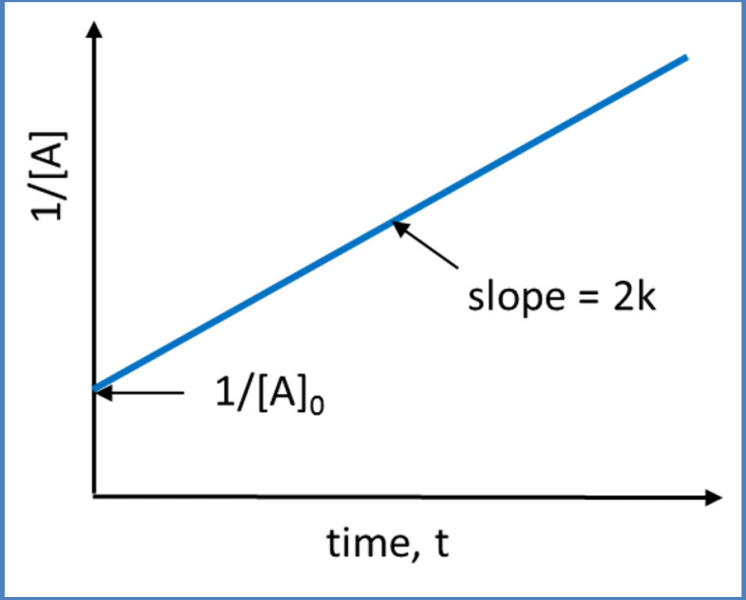
\includegraphics[scale = 0.35]{Rate Law Graph.png}
    \end{center}
    
    \subsection*{Establishing a rate law from measured reaction velocities}
    
    A different way of experimentally examining a rate law is by evaluating the 
    dependence of reaction velocity on concentrations. 

    If a reaction is \textbf{first order} in [A], then v will depend linearly on [A]. 
    If [A] doubles, then v will also double. 

    If a reaction is \textbf{second order} in [A], then doubling [A] will quadruple the 
    reaction velocity. 

    In general: 
    \begin{equation}
        v = [A]^{\alpha}
    \end{equation}

    Then for rate measurements made at two different concentrations: \\ \\
    \begin{equation}
        \ln(\frac{v_2}{v_1}) = \alpha \ln(\frac{[A]_2}{[A]_1})
    \end{equation}

    \subsection*{Behavior of more complex reaction schemes}

    Now, we want to consider events that are more complex than one step reactions. Consider 
    the following example: 

    \begin{center}
        
    \end{center}
   
    This gives the following equations:

    \begin{align*}
        \frac{d[A]}{dt} &= -k_1[A] \\ \\
        \frac{d[B}{dt} &= k_1[A] - k_2[B] \\ \\
        \frac{d[C]}{[dt]} &= k_2[B]  
        %\frac{1}{[A]} - \frac{1}{[A]_0} &= 2kt
    \end{align*}
    
    \newpage
    For another example: 

    \begin{center}
        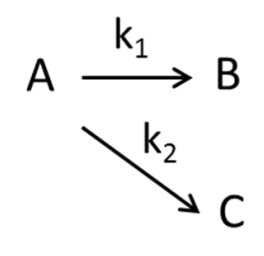
\includegraphics[scale = 0.5]{Complex Reaction.png}
    \end{center}

    The change in concentration as a function of time is given as: 

    \begin{align*}
        \frac{d[A]}{dt} &= -k_1[A] - k_2[A] = -(k_1 + k_2)[A] \\ \\
        \frac{d[B]}{dt} &= k_1[A] \\ \\
        \frac{d[C]}{[dt]} &= k_2[A]  
        %\frac{1}{[A]} - \frac{1}{[A]_0} &= 2kt
    \end{align*}

    \underline{Steady state assumptions for obtaining simple rate laws for complex reactions} \\ \\
    For complex reactions, dependence of the rate of the overall reaction (rate law) can depend on concentrations
    of species that do not contribue to the reaction itself.

    When sequential reactions are invovled, simplified rate laws can be obtained by assuming steady state conditions. 

    \textbf{Steady state} is when the intermediate species (that do not contribute to overall reaction stoichiometry) concentrations have reached
    constant value, at least momentarily.

    \begin{center}
        \( \frac{d[Intermediate]}{dt} = 0 \)
    \end{center}

    Consider the following equation: 
    \begin{equation}
        A \stackrel{k_1}{\underset{k_{-1}}{\rightleftharpoons}} B \stackrel{k_2} \longrightarrow C
    \end{equation}
    In this equation, the intermediate is B, and the overall reaction stoichiometry is \(A \longrightarrow C \).
    Based on equation 13, we can then state that: 

    \begin{align*}
        \frac{d[B]}{dt} &= k_1[A] - k_{-1}[B] - k_2[B] \\ \\
        &= k_1[A] - [B](k_{-1} + k_2) = 0
    \end{align*}

    Now rearrange to isolate [B]: 

    \begin{equation}
        [B] = \frac{k_1[A]}{k_2 + k_1} 
    \end{equation}

    Now go back to the original reaction scheme. The overall reaction velocity is \( v = \frac{d[C]}{dt} \), but 
    we know that \( \frac{d[C]}{dt} = k_2[B] \). Substituting [B] from equation 14 shows that: 

    \begin{equation}
        v = \frac{k_1 k_2 [A]}{k_2 + k_{-1}}    
    \end{equation}

    From the equation 15 above, this 2-step reaction behaves as first order in [A] at steady state. 
   
    \subsection*{Enzyme Kinetics under a steady-state assumption}

    The following model is used to treat kinetics of a simple unimolecular enzyme reaction: 
    \begin{equation}
        E + S \stackrel{k_1}{\underset{k_{-1}}{\rightleftharpoons}} ES \stackrel{k_{cat}} \longrightarrow E + P
    \end{equation}

    E is the free enzyme, S is the free/unbound substrate, ES is the enzyme-substrate complex, and P is the product. 
    \( \frac{k_1}{k_{-1}} \) describes how the tightly the enzyme binds the substrate. $K_{cat}$ describes the catalytic rate 
    constant for formation of P. 

    The velocity of the overall reaction is described by \( v = \frac{d[P]}{t} \). According to the rate law, $v = k_{cat}[ES]$. 
    [ES] is an intermediate, and so we need to replace [ES] by adopting steady state assumption (where $\frac{d[ES]}{dt} = 0$).

    \begin{align*}
        \frac{d[ES]}{dt} &= k_1[E][S] - (k_{-1} + k_{cat})[ES] = 0 \\ \\
        [ES] &= \frac{k_1[E][S]}{k_{-1} + k{cat}}
    \end{align*}

    Now plug in [ES] from above into $v = k_{cat}[ES]$ : 

    \begin{equation}
        v =  \frac{k_{cat}k_1[E][S]}{k_{-1} + k_{cat}}
    \end{equation}

    This equation is a start, but it only describes the reaction velocity in terms of the free enzyme concnetration. 
    In an experiment, we usually only have control over the total enzyme concnetratoin. We want to rewrite the equation 
    in terms of total enzyme concentration and in terms of the ratio of the reaction velocity to the maximum possible value ($[ES] = [E]_{total}$)
    The maximum velocity is $k_{cat} \times \text{max value for } [ES]$, which is: 

    \begin{equation}
        v_{max} = k_{cat}[E]_{total} = k_{cat}([ES] + [E])
    \end{equation}
    The ratio of reaction velocities relative to its maximum is given: 

    \begin{align*}
        \frac{v}{V_{max}} &= \frac{k_{cat}[ES]}{k_{cat}([E] + [ES])} \\ \\
        \frac{v}{V_{max}} &= \frac{[ES]}{([ES] + [E])} \\ \\
        \frac{v}{V_{max}} &= \frac{1}{1 + \frac{[E]}{[ES]}}
    \end{align*}

    Taking the previous equation \( [ES] = \frac{k_1[E][S]}{k_{-1} +  k_{cat}} \) and rearranging so that \\ it becomes \( \frac{[E]}{[ES]} = \frac{k_{-1} + k_{cat}}{k_1[S]}\), substitute this equation above to give:

    \begin{align*}
        \frac{v}{V_{max}} &= \frac{1}{1 + \frac{k_{-1} + k_{cat}}{k_1[S]}} \\ \\
        \frac{v}{V_{max}} &= \frac{[S]}{[S] + \frac{k_{-1} + k_{cat}}{k_1[S]}} \\ \\
        \frac{v}{V_{max}} &= \frac{[S]}{[S] + K_M} \longrightarrow K_M = \frac{k_{-1} + k_{cat}}{k_1}
    \end{align*}
    
    Or, we can also convert from fractional velocity to v using equation 18 for $V_{max}$:

    \begin{equation}
        v = \frac{k_{cat}[E]_{total}[S]}{[S] + K_M}
    \end{equation}

    \newpage

    \subsection*{Relaxation kinetics: how systems approach equilibrium}
    \subsubsection*{The T-Jump Method}
    The temperature jump method was developed to study fast reactions and their "relaxation" back towards equilibrium. 
    If energy is rapidly delivered to a solution containing reactant and product at equilibrium, the temperature of the 
    system can be heated nearly instantaneously. Recalling the \textbf{van't Hoff equation}, if $\Delta$H for the reaction is non-zero,
    then the equilibrium constant will be different at a new temperature. Then you can observe how fast the reaction returns to its 
    new equilibrium. 

    The speed at which equilbrium is achieved depends on the forward and backward rate constants of the reaction. 

    Consider a simple system:

    \begin{equation*}
        A \stackrel{k_1}{\underset{k_{-1}}{\rightleftharpoons}} B
    \end{equation*}

    Let $\textbf{x}$ be the distance of each species from equilibrium. $\bar{A}$ will be $[A]_{equilbrium}$ at the new temperature, same for $\bar{B}$.
    The concentrations of A and B are related to the equilibrium conc. by: 
    \begin{align*}
        [A] &= \bar{A} + x \\
        [B] &= \bar{B} - x
    \end{align*}
    
    Now examine the approach to equlibrium by writing an equation for time dependence of \textbf{x}. 

    \begin{align*}
        \frac{d[A]}{dt} &= \frac{d[\bar{A} + x]}{dt} = \frac{dx}{dt} \\ \\ 
        \frac{d[A]}{dt} &= -k_1[A] + k_{-1}[B] \\ \\
        \frac{d[A]}{dt} &= -k_1[\bar{A} + x] + k_{-1}[\bar{B} - x] \\ \\
        &= k_{-1}\bar{B} - k_{-1}\bar{A} - x(k_1 + k_{-1})
    \end{align*}

    The term \(k_{-1}\bar{B} - k_{-1}\bar{A} = 0 \) because \( \frac{\bar{B}}{\bar{A}} = K = \frac{k_1}{k_{-1}} \)

    So, after setting the above to 0, the equation yields: 

    \begin{equation}
        \frac{dx}{dt} = -(k_1 + k_{-1})x
    \end{equation}

    X follows first order kinetics. Skipping the familiar detials for handling a first order differential equation: 

    \begin{equation}
        x = x_o^{-(k_1 + k_{-1})} \text{ and } \ln(\frac{x}{x_0}) = -(k_1 + k_{-1})t
    \end{equation}

    Convert these to even more general forms:

    \begin{equation}
        x = x_0e^{\frac{-t}{\tau}} \text{ and } \ln(\frac{x}{x_0}) = \frac{-t}{\tau}
    \end{equation}
    
    where \( \tau = \frac{1}{k_1 + k_{-1}} \)

    \begin{center}
        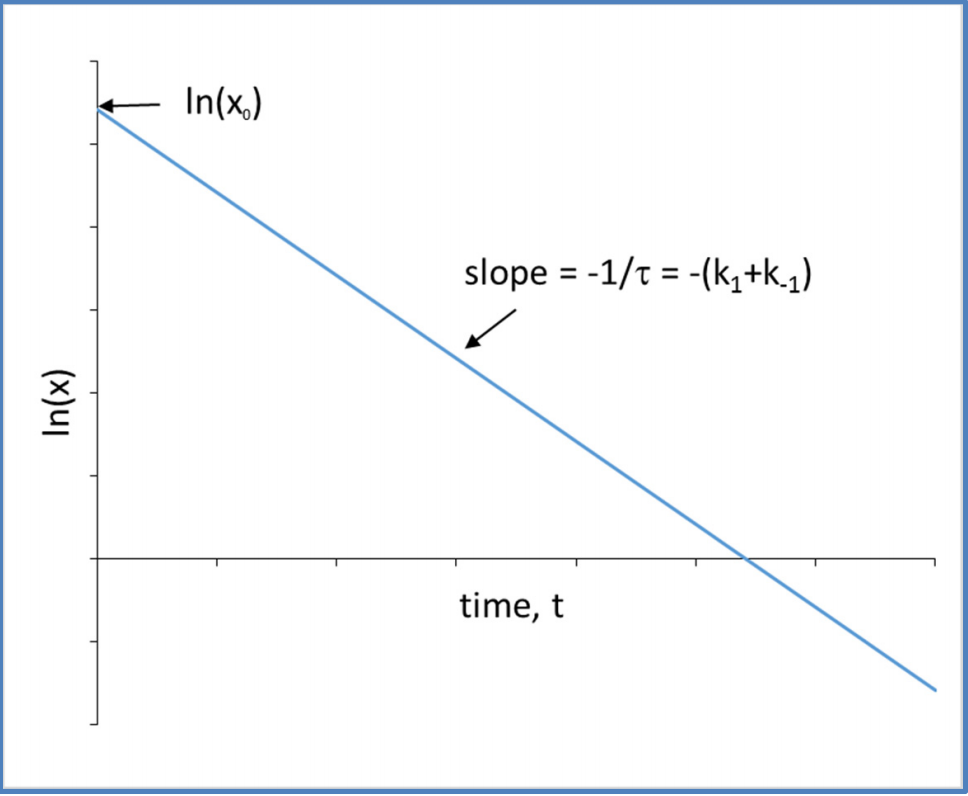
\includegraphics[scale = 0.4]{ln(x) vs. time.png}
    \end{center}
    
    If you can find [A] or [B] as a function of time, then you can also find \textbf{x} as a function of time. 

    \textbf{x} = $[A] - \bar{A}$ = $\bar{B} - [B]$

    You can use this to measure $\tau$, and thus also \(k_1 + k_{-1} \)

    \begin{align*}
        1/\tau &= k_1 + k_{-1} \text{ and } k_1 = Kk_{-1} \\ \\ 
        1/\tau &= Kk_{-1} + k_{-1} = (K+1)k_{-1}
    \end{align*}

    \begin{equation*}
        k_{-1} = \frac{1}{\tau(K + 1)} \text{ and } k_1 = \frac{K}{\tau(K + 1)}
    \end{equation*}

\subsubsection*{Higher Order Reactions Approaching Equilibrium}

Now consider this second order reversible reaction:

\begin{equation*}
    A + B \stackrel{k_1}{\underset{k_{-1}}{\rightleftharpoons}} C
\end{equation*}

There is only one transformation, st he distance can still be described by \textbf{x}:

\begin{align*}
    [A] &= \bar{A} + x \\ \\ 
    [B] &= \bar{B} + x \\ \\
    [C] &= \bar{C} - x
\end{align*}

We can use the same approach from the above to describe the change in concentrations: 

\begin{align*}
    \frac{d[A]}{dt} &= \frac{d\bar{A} + x}{dt} = \frac{dx}{dt} \\ \\
    \frac{d[A]}{dt} &= -k_1(\bar{A} + x)(\bar{B} + x) + k_{-1}(\bar{C} - x) \\ \\ 
    &= k_{-1}\bar{C} - k_1\bar{A}\bar{B} - x(k_1(\bar{A} + \bar{B}) + k_{-1}) - k_1x^2
\end{align*}

\( k_{-1}\bar{C} - k_1\bar{A}\bar{B} \) cancels to 0, and if we are close enough to equilibrium then x is small, so we can neglect the $x^2$ term. 
So, 

\begin{equation}
    \frac{dx}{dt} = -(k_1(\bar{A} + \bar{B}) + k_{-1})x
\end{equation}

So, the distance from equilibrium x shows first order behavior close to equilibrium, with \( \tau = \frac{1}{k_1(\bar{A} + \bar{B}) + k_{-1}} \)

\newpage

\subsection*{Kinetics from Single Molecule Studies}
For a unimolecular event, we can get a sense for the rate constant by looking at how long the molecule
persists in its current state before undergoing a reaction. 

Think of this as the "waiting time" before a reaction or confroational change occurs. 
While reactions are random, the average waiting time should be shorter for a process with a higher rate constant. 

Consider \( A \longrightarrow B \) with rate constant k. 

How long before any molecule A turns into B? Treat the reaction in bulk: 

\begin{equation}
    \frac{A}{A_0} = e^{\frac{-t}{\tau}} \text{ where } \tau = \frac{1}{k}
\end{equation}

$\frac{A}{A_0} $ can be considered the probability that any molecule A will \textbf{not} convert at time t. 

The probability that molecule A reacts precisely at time t is \( P(A)_{react} = \frac{1}{\tau} e^{\frac{-t}{\tau}} \).

To get the average time at which a molecule of A reacts (aka waiting time), we need
to get the average value of t by weighting all possible values of t by probability of reaction at time t. 

\textbf{To do this}, multiply t by the probability of reaction at time t, then integrate from t = 0 to infinity. 

\begin{equation}
    \text{waiting time} = \int_{t = 0}^{t = \infty}(t(\frac{1}{\tau})e^{\frac{-t}{\tau}})dt
\end{equation}

If we can measure how long it takes a single molecule to undergo a transition,then we have measured $\tau$. 

\newpage

\section*{Chapter 16: Kinetic Theories and Enzyme Catalysis}
Now we want to look at what determines the rate constant, k. What makes some reactions innately fast or slow?
There are two main models that try to explain the mechanisms of chemical reactions and their rate constants. 

\subsection*{The Arrhenius Equaton}

This is often used to discuss reaction rates in terms of \textbf{molecular collisions}. 
The rate constant k is determined by:

\begin{equation}
    k = Ae^{-\frac{E_a}{RT}}
\end{equation}

A is the \textbf{frequency factor} and $E_a$ is an \textbf{activation energy}. 
We already know that the frequency of collisions in a reaction is dependent on concentrations. 
The frequency factor in the equation for k accounts for other phenomena ie. the dependence of molecular
velocities and consequently collision rates on temperature, and the dependence of reaction probability on 
the orientation of the colliding molecules. 

\textbf{$E_a$} describes a lower bound for energy that reactants must have for reaction to occur. Why does $E_a$ 
enter the equation for k as an exponential term? \textbf{Boltzmann Distrbution!}

If \( N(E) \propto e^{\frac{-E}{RT}} \), then we can find the fraction of molecules having energy at least as high as $E_a$ by 
\textbf{taking the ratio of area that falls under the curve and has E $\geq$ $E_a$} divided by entire area under the curve. 

\begin{align*}
    \frac{\int_{E_a}^{\infty}  e^{\frac{-E}{RT}}}{\int_{0}^{\infty}  e^{\frac{-E}{RT}}} &= \frac{-RTe^{\frac{-E}{RT}} |_{E_a}^{\infty}}{-RTe^{\frac{-E}{RT}}|_{0}^{\infty}} \\ \\
    \frac{e^{-\frac{E_a}{RT}}}{1} &= e^{-\frac{E_a}{RT}}
\end{align*}


\end{document}
